\PassOptionsToPackage{hyphens}{url}
\documentclass{ieeeaccess}

\usepackage{cite}
\usepackage{amsmath,amssymb,amsfonts}
\usepackage{booktabs}
\usepackage{graphicx}
\usepackage{tabularx}
\usepackage{textcomp}
\usepackage{url}
\usepackage{placeins}
\usepackage{balance}
\usepackage{needspace}
\usepackage{siunitx}
\sisetup{detect-all,group-digits=false,retain-explicit-plus=true}

\graphicspath{{../results/figures/}}
% Figures are authored as editable SVG files. The vector-PDF mirrors used by
% pdfLaTeX are generated at their final publication widths.
\newcommand{\widefigwidth}{\textwidth}
\newcommand{\settableformat}{%
  \fontsize{8}{10}\selectfont
  \setlength{\tabcolsep}{4pt}%
  \renewcommand{\arraystretch}{1.12}%
  \setlength{\heavyrulewidth}{0.7pt}%
  \setlength{\lightrulewidth}{0.4pt}%
}
% Generated by scripts/revision_analysis.py; do not edit.
\newcommand{\CondGapMean}{+0.035}
\newcommand{\CondGapLo}{+0.030}
\newcommand{\CondGapHi}{+0.040}
\newcommand{\AllGapMean}{+0.030}
\newcommand{\AllGapLo}{+0.025}
\newcommand{\AllGapHi}{+0.034}
\newcommand{\CondTargetMean}{+0.035}
\newcommand{\AllTargetMean}{+0.030}
\newcommand{\DatasetMean}{+0.030}
\newcommand{\MetaMean}{+0.030}
\newcommand{\MetaLo}{+0.014}
\newcommand{\MetaHi}{+0.046}
\newcommand{\MetaPredLo}{-0.010}
\newcommand{\MetaPredHi}{+0.071}
\newcommand{\MetaI}{74.7}
\newcommand{\AllDatasetMean}{+0.024}
\newcommand{\AllMetaMean}{+0.024}
\newcommand{\AllMetaLo}{+0.009}
\newcommand{\AllMetaHi}{+0.039}
\newcommand{\AllMetaPredLo}{-0.016}
\newcommand{\AllMetaPredHi}{+0.064}
\newcommand{\AllMetaI}{83.7}
\newcommand{\CondMedian}{+0.031}
\newcommand{\CondIQRLo}{+0.017}
\newcommand{\CondIQRHi}{+0.053}
\newcommand{\AllMedian}{+0.026}
\newcommand{\AllIQRLo}{+0.014}
\newcommand{\AllIQRHi}{+0.046}
\newcommand{\CondPositive}{89.9}
\newcommand{\CondGtOne}{83.3}
\newcommand{\CondGtTwo}{71.0}
\newcommand{\AllPositive}{89.9}
\newcommand{\AllGtOne}{81.9}
\newcommand{\AllGtTwo}{66.7}
\newcommand{\CSPGapMean}{+0.036}
\newcommand{\CSPGapLo}{+0.029}
\newcommand{\CSPGapHi}{+0.044}
\newcommand{\TSGapMean}{+0.033}
\newcommand{\TSGapLo}{+0.029}
\newcommand{\TSGapHi}{+0.038}
\newcommand{\AllCSPGapMean}{+0.031}
\newcommand{\AllCSPGapLo}{+0.024}
\newcommand{\AllCSPGapHi}{+0.038}
\newcommand{\AllTSGapMean}{+0.029}
\newcommand{\AllTSGapLo}{+0.025}
\newcommand{\AllTSGapHi}{+0.032}
\newcommand{\RankChangeN}{19}
\newcommand{\CondRankChangeN}{19}
\newcommand{\RankChangePct}{13.8}
\newcommand{\ThresholdSeventyN}{16}
\newcommand{\ThresholdSeventyFiveN}{31}
\newcommand{\AllRankChangeN}{14}
\newcommand{\AllRankChangePct}{10.1}
\newcommand{\AllThresholdSeventyN}{13}
\newcommand{\AllThresholdSeventyFiveN}{22}
\newcommand{\DriftRobustBeta}{-0.0001}
\newcommand{\DriftRobustLo}{-0.0050}
\newcommand{\DriftRobustHi}{+0.0047}
\newcommand{\DriftRobustP}{0.9530}
\newcommand{\DriftInfluentialN}{91}
\newcommand{\CondMatchedTriangleSE}{0.0180}
\newcommand{\StrictMatchedTriangleSE}{0.0221}
\newcommand{\CondMatchedRowQSE}{0.0519}
\newcommand{\StrictMatchedRowQSE}{0.0578}
\newcommand{\UniformTotalMean}{+0.035}
\newcommand{\UniformTotalLo}{+0.030}
\newcommand{\UniformTotalHi}{+0.040}
\newcommand{\UniformCountMean}{+0.025}
\newcommand{\UniformCountLo}{+0.022}
\newcommand{\UniformCountHi}{+0.029}
\newcommand{\UniformCompositionMean}{+0.009}
\newcommand{\UniformCompositionLo}{+0.005}
\newcommand{\UniformCompositionHi}{+0.014}
\newcommand{\StrictTotalMean}{+0.053}
\newcommand{\StrictTotalLo}{+0.045}
\newcommand{\StrictTotalHi}{+0.061}
\newcommand{\StrictCountMean}{+0.040}
\newcommand{\StrictCountLo}{+0.035}
\newcommand{\StrictCountHi}{+0.045}
\newcommand{\StrictCompositionMean}{+0.013}
\newcommand{\StrictCompositionLo}{+0.006}
\newcommand{\StrictCompositionHi}{+0.020}
\newcommand{\AllFlipMarginOneN}{1}
\newcommand{\AllFlipCSPtoTSN}{10}
\newcommand{\AllFlipTStoCSPN}{4}
\newcommand{\AllMetaHKLo}{+0.009}
\newcommand{\AllMetaHKHi}{+0.039}
\newcommand{\CondFlipMarginOneN}{6}
\newcommand{\CondFlipCSPtoTSN}{15}
\newcommand{\CondFlipTStoCSPN}{4}
\newcommand{\CondMetaHKLo}{+0.014}
\newcommand{\CondMetaHKHi}{+0.047}
\newcommand{\StrictFutureMean}{+0.017}
\newcommand{\StrictFutureLo}{+0.007}
\newcommand{\StrictFutureHi}{+0.026}
\newcommand{\MaBlockCond}{+0.036}
\newcommand{\MaBlockAll}{+0.033}
\newcommand{\MaDayCond}{+0.039}
\newcommand{\MaDayAll}{+0.019}
\newcommand{\MaDayBA}{+0.033}
\newcommand{\MaDayBALo}{+0.019}
\newcommand{\MaDayBAHi}{+0.047}

% Generated by scripts/donor_sampling_uncertainty.py; do not edit.
\newcommand{\CondCompDrawSE}{0.0007}
\newcommand{\CondCompParticipantSE}{0.0022}
\newcommand{\StrictCompDrawSE}{0.0012}
\newcommand{\StrictFutureDrawSE}{0.0009}
\newcommand{\CondCountShare}{73}
\newcommand{\CondCompShare}{27}
\newcommand{\StrictCountShare}{76}
\newcommand{\SharedSeedPairs}{3}
\newcommand{\SubjectTPairs}{135}


\newcommand{\AUC}{\mathrm{AUC}}
\newcommand{\LOSO}{\mathrm{LOSO}}
\newcommand{\EXP}{\mathrm{EXP}}

\begin{document}

\history{}
\doi{}
\vol{14}
\year{2026}

\title{LOSO versus Chronological Validation in Longitudinal BCI}

\author{\uppercase{Yiming Shen}\authorrefmark{1}}
\address[1]{Department of Mathematics, University of Massachusetts Boston,
Boston, MA 02125 USA (e-mail: yiming.shen001@umb.edu)}
\markboth
{Shen: LOSO versus Chronological Validation in Longitudinal BCI}
{Shen: LOSO versus Chronological Validation in Longitudinal BCI}
\corresp{Corresponding author: Yiming Shen (e-mail: yiming.shen001@umb.edu).}

\begin{abstract}
Motor-imagery brain--computer interfaces used over many sessions are often
retrained before each session, using only the sessions recorded so far.
Leave-one-session-out (LOSO) validation instead trains on all other sessions,
including later ones, whereas expanding-window validation uses only earlier
sessions. We compared the two protocols on identical test sessions in six binary
motor-imagery datasets with 138 participants, using common-spatial-pattern and
tangent-space decoders with fixed configurations. Where LOSO could also train on
later sessions, its participant-weighted mean area under the receiver operating
characteristic curve was 0.035 higher than under expanding-window validation
(95\% confidence interval [0.030, 0.040]). The difference was positive in every
dataset but varied in size. When the LOSO pool was sampled down to the
expanding window's number of training sessions, most of the gap disappeared.
The dataset-level order of the two decoders did not change, and
participant-level ranking changes occurred mainly near ties. We provide
reporting specifications and a chronological cross-validator for the Mother of
All BCI Benchmarks. Longitudinal benchmarks should report a chronological
estimate alongside LOSO and judge decoder rankings by their score margins.
\end{abstract}

\begin{keywords}
Brain--computer interfaces, cross-session decoding, electroencephalography,
longitudinal evaluation, motor imagery, prospective validation.
\end{keywords}

\titlepgskip=-21pt
\maketitle
\raggedbottom

\section{Introduction}
\label{sec:introduction}
\PARstart{R}{epeated} use of motor-imagery brain--computer interfaces (BCIs)
means decoding each new session with the labeled sessions collected so far.
In one rehabilitation system, for example, each session on a new day began
with collecting calibration data and training the decoder
\cite{hernandezrojas2022fes}. The EEG itself varies from session to session.
Changes in concentration alter it between days and lower intention-detection
rates \cite{maswanganyi2022intersession}, and caffeine lowers resting alpha and
beta power in the band used for online control \cite{meng2017softdrinks}. Such
changes have motivated decoder adaptation and the reuse of earlier sessions
\cite{krauledat2008zero,wimpff2025continual}. For a decoder retrained before
each session, evaluation has to ask how well it decodes the next session from
the labeled sessions available at that point. The answer matters whenever a
benchmark is used to describe performance during repeated use or to choose
between candidate decoders.

Leave-one-session-out (LOSO) validation trains on all of a participant's
sessions except the target, including sessions recorded after it.
Expanding-window validation trains only on earlier sessions, following the
rolling-origin principle \cite{tashman2000outofsample}. The two protocols can
therefore score identical test trials under different information conditions:
the completed recording trajectory for LOSO, and the history available before
the target for the expanding window. Moving from prior history to the LOSO pool
alters both the number and the composition of training sessions, and how much
this moves the score is an empirical question. In subject-independent studies
the same acronym often denotes leave-one-subject-out validation
\cite{keutayeva2023attention,sugata2026fear}; here it always refers to sessions.

The reported difference also depends on which targets enter the average. At the
final session the two protocols use the same training set. With deterministic
fitting, this target therefore contributes a zero difference, and its weight in
the average depends on trajectory length. Averages over targets where the
training sets differ cover a different part of the trajectory than averages
that include the final session.

A recent protocol for trustworthy EEG decoding controls hyperparameter search
and training randomness within LOSO evaluation, but does not vary which
sessions are available for training \cite{borra2025trustworthy}. Other studies
use session order directly, in session-level protocol comparisons
\cite{egger2024chrono} and in continual fine-tuning and adaptation that train on
earlier data as it accumulates \cite{wimpff2025continual,haxel2026edapt}.
Building on these studies, we measure the paired difference across recording
designs, compare it with a session-count-matched reference, and ask whether it
changes decoder ordering. A protocol can shift two decoders' scores by similar
amounts and leave their order intact, while small differences near a tie can
reverse it. Throughout, the participant, the test trials, and the decoder
configurations stay fixed; only the eligible training sessions change.

We compare fixed common-spatial-pattern and tangent-space decoder
configurations, fitted separately under each protocol, on identical test
sessions in six binary motor-imagery datasets with 138 participants. A
reference drawn uniformly from the LOSO pool matches the expanding window's
number of training sessions. We quantify the differences across datasets and
target-averaging definitions, and assess decoder ordering together with
within-protocol score margins. We also provide reporting specifications and a
chronological cross-validator compatible with the Mother of All BCI Benchmarks
(MOABB). In every dataset, LOSO gave the higher mean score and the two decoders
kept the same order.

\section{Related Work}
\label{sec:related}
Tashman's analysis of out-of-sample forecasting links performance assessment
to forecast origins, model updates, and the observations available for training
\cite{tashman2000outofsample}. Rolling-origin evaluation provides the temporal
basis for successive prediction with an expanding history. His discussion also
distinguishes choices about recalibration and repeated test origins from the
selection of a forecasting method. Time-series cross-validation,
leave-future-out validation, and model assessment under temporal distribution
shift further examine how training and test periods define the prediction task
\cite{bergmeir2012crossvalidation,burkner2020leavefuture,han2024temporal}.

MOABB standardizes datasets, pipelines, and evaluation interfaces, including
cross-session evaluation within a participant \cite{jayaram2018moabb}.
Borra \emph{et al.} address configuration search and training variability
through hyperparameter optimization and repeated random initialization within
participant-specific LOSO evaluation \cite{borra2025trustworthy}.
Varoquaux \emph{et al.} examine cross-validation and model selection for brain
decoders \cite{varoquaux2017assessing}, while Brookshire \emph{et al.} study
subject-level separation in EEG \cite{brookshire2024leakage}. Sugata
\emph{et al.} report over 98\% accuracy under 10-fold cross-validation and about
37\% under leave-one-subject-out validation for the same EEG model, and attribute
much of the gap to leakage between windows cut from the same trials
\cite{sugata2026fear}. For motor imagery, Li \emph{et al.} report 85.84\% under
pooled 10-fold cross-validation and 79.95\% under session-to-session hold-out for
one model on BCI Competition IV-2a \cite{li2026fbda}.
Carrara and Papadopoulo introduce pseudo-online evaluation in MOABB, including
within-session tests in which test trials follow training trials
\cite{carrara2024pseudoonline}. These designs control different aspects of
performance evidence: model selection, participant independence, and temporal
ordering.

Session-level temporal comparisons and decoder adaptation provide complementary
evidence. Egger \emph{et al.} compare five decoding strategies, including LOSO
and expanding-history training, in a repeated study of executed hand gestures
\cite{egger2024chrono}. Wimpff \emph{et al.} evaluate continual motor-imagery
fine-tuning restricted to earlier sessions \cite{wimpff2025continual}.
Haxel \emph{et al.} combine population-level pretraining with trial-wise
supervised adaptation across nine datasets and three BCI paradigms
\cite{haxel2026edapt}. Riemannian alignment and session-selection methods
address the use of donor recordings
\cite{zanini2018transfer,sung2024sessiontransfer,shen2026confidence}.
SessionNet combines multi-session motor-imagery data through a
similarity-weighted ensemble \cite{lee2020sessionnet}, and source-selection
methods choose which source data to transfer \cite{heskebeck2026source}.
Incremental CSP updating \cite{jiang2020adaptivecsp}, synchronized
self-training, and nonstationary attention
\cite{chen2025synchronized,guo2025crosssession} adapt the decoding pipeline to
nonstationary recordings.

Training-set size and validation choices also affect the interpretation of
decoder comparisons. \'Sliwowski \emph{et al.} examine training-set size and
recording period through complementary learning-curve designs in one ECoG user
followed over 43 sessions \cite{sliwowski2023datasetsize}. Schroeder
\emph{et al.} compare pseudo-online, leave-one-block-out, and k-fold evaluation
across three passive-BCI datasets, reporting changes in accuracy and relative
classifier performance \cite{schroeder2025crossval}. Chang \emph{et al.} compare
random, leave-one-subject-out, and nested leave-one-subject-out evaluation on a
motor-imagery dataset \cite{chang2026validation}. Their subject-generalization
comparisons address a different test population from session-history
comparisons within the same participant. These studies connect performance
estimates to both the available training data and the population over which
predictions are evaluated.

\Needspace{7\baselineskip}
\section{Evaluation Targets and Estimands}
\label{sec:estimands}
\subsection{One Target, Two Information Sets}
For participant $i$ with ordered sessions $0,\ldots,T_i-1$, the donor sets at
target session $t$ are
\begin{align}
S_{\LOSO}(t) &= \{0,\ldots,T_i-1\}\setminus\{t\},\\
S_{\EXP}(t) &= \{0,\ldots,t-1\}.
\end{align}
Both protocols reserve every trial from session $t$ for testing. Performance is
measured by the area under the receiver operating characteristic curve (AUC).
For decoder $m$, the paired contrast is
\begin{equation}
\Delta_{i,t,m}=\AUC^{\LOSO}_{i,t,m}-\AUC^{\EXP}_{i,t,m}.
\end{equation}
Evaluation begins at $t=1$, when at least one prior session exists. At the final
target, the two donor sets coincide, so $\Delta_{i,T_i-1,m}=0$.
Figure~\ref{fig:logic} shows the two information sets and the two sets of
targets that are averaged.

\begin{figure*}[!t]
\centering
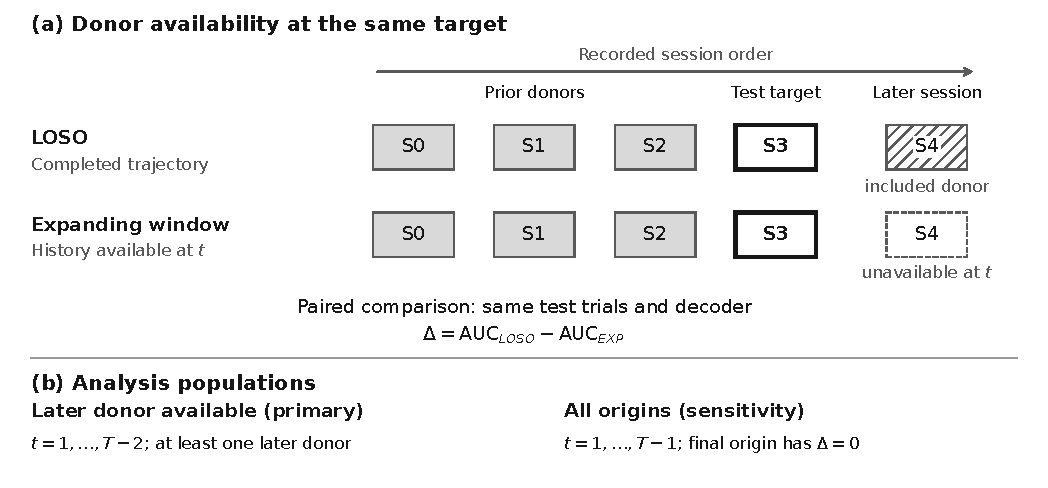
\includegraphics[width=\widefigwidth]{fig0_protocol_logic.pdf}
\caption{Information sets for the paired evaluation. (a) At the same early target,
LOSO trains on prior sessions and a later session, whereas the expanding window
uses only the history already available. The test trials and decoder are identical.
(b) The primary estimand averages the targets at which a later donor is
available; the all-origin sensitivity summary also includes the final origin,
where the donor sets coincide and the difference is zero.}
\label{fig:logic}
\end{figure*}

\subsection{Primary and Sensitivity Estimands}
Let $N=138$ and let $m$ index the two fixed decoder configurations, CSP+LDA and
TS+LR. The primary estimand covers the targets at which the two protocols can
differ, that is, targets with at least one later session available to LOSO. We
first average targets and decoders within participant, then give each
participant equal weight:
\begin{equation}
\theta_{\mathrm{future}>0}=\frac{1}{N}\sum_i
\frac{1}{2(T_i-2)}\sum_m\sum_{t=1}^{T_i-2}\Delta_{i,t,m}.
\end{equation}
Target-weighted summaries instead give each participant--target pair equal
weight after averaging decoders. Dataset-weighted summaries average the six
dataset means equally.

As a sensitivity summary, the all-origin estimand also includes the final
target $t=T_i-1$, where the two training sets coincide and $\Delta=0$ by
construction. Writing $\bar\Delta_i$ for the within-participant average over
targets and both decoders,
\begin{equation}
\bar\Delta_{i,\mathrm{all}}
=\frac{T_i-2}{T_i-1}\,\bar\Delta_{i,\mathrm{future}>0},
\label{eq:zero-scaling}
\end{equation}
so the all-origin mean is the conditional mean rescaled, not a second,
independent comparison.

\section{Methods}
\label{sec:methods}
We evaluate offline retraining on the recorded binary motor-imagery
trajectories. Donor sessions are fully labeled, AUC is the primary outcome, and
adaptation within a session is outside our scope. The primary analysis compares fixed CSP+LDA and TS+LR configurations across six
datasets and 138 participants. Appendix~\ref{app:eegnet} adds a single-seed
EEGNet run on Stieger2021 (62 participants) with a three-seed check on a
12-participant subset.
\subsection{Datasets and Time Units}
We used the six public datasets in Table~\ref{tab:data}. Each provides binary
motor-imagery labels, at least three chronologically ordered recording units per
participant, and complete results for both decoders. Together they contain 138
participants.

Zhou2016 and Zhou2020 are distinct datasets \cite{zhou2016trial,zhou2021relative}.
Ma2020 records right-hand and right-elbow imagery \cite{ma2020samejoint}; the
remaining datasets use left- and right-hand imagery. The unit of time is the
session or recording day as released by the source, except for Ma2020, where
the primary analysis uses the 15 released blocks and a sensitivity analysis
regroups them into their three recording days. One unit does not mean the same
elapsed time in different studies, and exact intervals were unavailable for
BNCI2014\_004, so we interpret session lag within each dataset and keep the
source's ordering.

\begin{table*}[!t]
\centering
\settableformat
\caption{Longitudinal motor-imagery datasets in the audit. Channel counts refer to
EEG channels retained by the audited loader.}
\label{tab:data}
\begin{tabularx}{\textwidth}{@{}>{\raggedright\arraybackslash}X S[table-format=2.0] >{\raggedright\arraybackslash}Xrl@{}}
\toprule
\textbf{Dataset} & {\textbf{Participants}} & \textbf{Ordered units} & \textbf{EEG channels} & \textbf{Source}\\
\midrule
BNCI2014\_004 & 9 & 5 sessions & 3 bipolar & \cite{tangermann2012review}\\
Zhou2016 & 4 & 3 sessions & 14 & \cite{zhou2016trial}\\
Zhou2020 & 20 & 6 or 7 sessions & 41 or 26 & \cite{zhou2021relative}\\
Kumar2024 & 18 & 6 sessions & 22 & \cite{kumar2024transfer}\\
Ma2020 & 25 & 15 blocks in 3 days & 62 & \cite{ma2020samejoint}\\
Stieger2021 & 62 & 7 or 11 sessions & 60 retained & \cite{stieger2021continuous}\\
\bottomrule
\end{tabularx}
\end{table*}

Every recording was band-pass filtered from 8 to 35 Hz, resampled to 128 Hz, and
epoched over $[0,3)$ s relative to the task cue, giving 384 samples per trial.
Ma2020 CNT files were loaded after removing horizontal and vertical
electrooculography channels, the mastoid reference, and optional electromyography
channels, leaving 62 scalp EEG channels.
Filtering, resampling, and epoching used fixed settings that did not depend on
target-session labels or performance. The classical pipelines used no
participant-wide or cross-session normalization. EEGNet's donor-only channel
standardization is specified in Appendix~\ref{app:eegnet}.

\subsection{Decoders and Information Isolation}
We used two established decoder families that rest on different feature
geometries and have complete results in all six datasets. Common spatial
patterns with linear discriminant analysis (CSP+LDA) is a supervised
spatial-filter pipeline; tangent-space features with logistic regression
(TS+LR) works with covariance geometry in a tangent space. Both are standard in
motor imagery \cite{lotte2018review}, and the tangent-space approach follows
the Riemannian framework reviewed in
\cite{congedo2017riemannian,yger2017riemannian}. Their settings are
deterministic and fixed, so the comparison stays on the evaluation protocol and
not on decoder search.

CSP+LDA used $\min(8,p)$ common spatial pattern (CSP) components for $p$ channels,
reduced to the next lower even number when required. CSP used Ledoit--Wolf
regularization, and linear discriminant analysis used the \texttt{lsqr} solver
with automatic shrinkage \cite{blankertz2008csp}. TS+LR estimated a Ledoit--Wolf
covariance for each trial, learned the affine-invariant tangent-space reference
from the donor covariances, and fitted $L_2$ logistic regression with $C=1$ and
the \texttt{lbfgs} solver \cite{barachant2012riemann}. All hyperparameters were
held fixed across protocols.

We fitted every combination of participant, target, protocol, and decoder from
scratch. CSP filters, LDA weights, the tangent-space reference, and the
logistic-regression weights were all estimated from donor trials; the target
session was used only for scoring. AUC was the primary endpoint, and the
Ma2020 day-level sensitivity analysis also reported balanced accuracy.

\subsection{Statistical Analysis}
For the primary analysis we took participant-level conditional means and
computed two-sided one-sample $t$ intervals, with Wilcoxon signed-rank tests as
a check. The all-origin summary was treated the same way. Target-weighted
intervals came from 5,000 participant-cluster bootstrap resamples, and dataset
means were summarized with participant-level intervals and equal-dataset
weighting. We also left out each dataset in turn and recomputed the participant-weighted
estimate for both summaries.

We pooled the six dataset means in a random-effects synthesis, using each
dataset's participant-level mean and sampling variance and estimating the
between-dataset variance by restricted maximum likelihood. The summary interval
used a $t$ reference across the six datasets, and the prediction interval added
the between-dataset variance to the uncertainty of the mean
\cite{higgins2009reevaluation}. Heterogeneity was summarized by $I^2$. The exact
formulas and a Hartung--Knapp--Sidik--Jonkman residual-scale sensitivity
analysis \cite{rover2015hartung} are in Appendix~\ref{app:uncertainty}.
Intervals and tests are unadjusted for multiple comparisons; secondary contrasts
and sensitivity checks are reported as descriptive analyses.

To see whether the protocol changes decisions, we looked at the participant
distribution of $\Delta$ and at which decoder scored higher for each participant
under each protocol. For every ranking change we recorded its direction and
whether it survived when both within-protocol decoder differences exceeded
0.005, 0.01, or 0.02 AUC; these thresholds say how close to a tie the two scores
were. Two absolute AUC thresholds, 0.70 and 0.75, appear in the appendix as
illustrations.

\subsection{Session-Count-Matched Reference}
\label{sec:matched}
At target $t$, LOSO trains on $T_i-1$ sessions and the expanding window on $t$.
The session-count-matched reference draws $t$ sessions at random from the LOSO
donor pool $S_{\LOSO}(t)$, fits the decoder on them, and averages the AUC over
five draws from a participant-specific seed. This puts the complete donor set,
the matched reference, and the prior-history set on the same targets, and on
every target with a later donor the contrast splits as
\begin{align}
\AUC_{\LOSO}-\AUC_{\EXP}={}&
(\AUC_{\LOSO}-\AUC_{\mathrm{matched}})\nonumber\\
&+(\AUC_{\mathrm{matched}}-\AUC_{\EXP}).
\label{eq:partition}
\end{align}
The first term compares the complete donor set with $t$ donors drawn from the
same pool. The second compares those $t$ donors with the $t$ prior sessions.
Both components belong to this particular reference, which draws sessions
uniformly and matches the number of sessions, not the number of trials. A second
arm drew its $t$ sessions from the strictly later sessions only; it exists when
$T_i-1-t\geq t$, that is, on early targets with $t\leq(T_i-1)/2$. Intervals for
the sampled arms condition on the realized draws, and
Appendix~\ref{app:uncertainty} bounds the donor-sampling standard error.

\subsection{Temporal-Unit and Supporting Analyses}
For Ma2020 we also concatenated blocks 1--5, 6--10, and 11--15 into three
recording days, kept every trial, refitted both decoders, and recomputed the
conditional and all-origin summaries. At the block level the chronological arm
updates the decoder before each block using the earlier blocks; at the day
level it updates before each day using the earlier days and scores all trials of
that day. The unit therefore decides when the decoder is updated, what it is
tested on, and which targets enter the average.

Two further training policies, the immediately previous session only and the
first session only, give reference points. A target-position analysis relates
the conditional contrast to the number of later sessions LOSO had available
within each dataset. As a drift proxy we used the affine-invariant Riemannian
distance between the unconditional mean trial covariance matrices of sessions
$t-1$ and $t$,
standardized within dataset, and regressed the target-level contrast on it,
adjusting for target index, decoder, and dataset with participant-clustered
standard errors.

\section{Results}
\label{sec:results}
\subsection{Higher Mean LOSO Scores on Identical Test Sessions}
At the 1,001 participant--targets where LOSO had at least one later session
available, participant-weighted mean AUC was 0.766 under LOSO and 0.731 under
the expanding window, a paired difference of \CondGapMean{} AUC (95\% CI
[\CondGapLo{}, \CondGapHi{}]). Weighting targets instead of participants gave
much the same. Adding each participant's final target, where the two training
sets coincide and the difference is zero by construction, pulled the average
down to \AllGapMean{} AUC (95\% CI [\AllGapLo{}, \AllGapHi{}]).
Figure~\ref{fig:estimands}(b) shows the participant distributions, and
Table~\ref{tab:estimands} gives the aggregation analyses.

\begin{figure*}[!t]
\centering
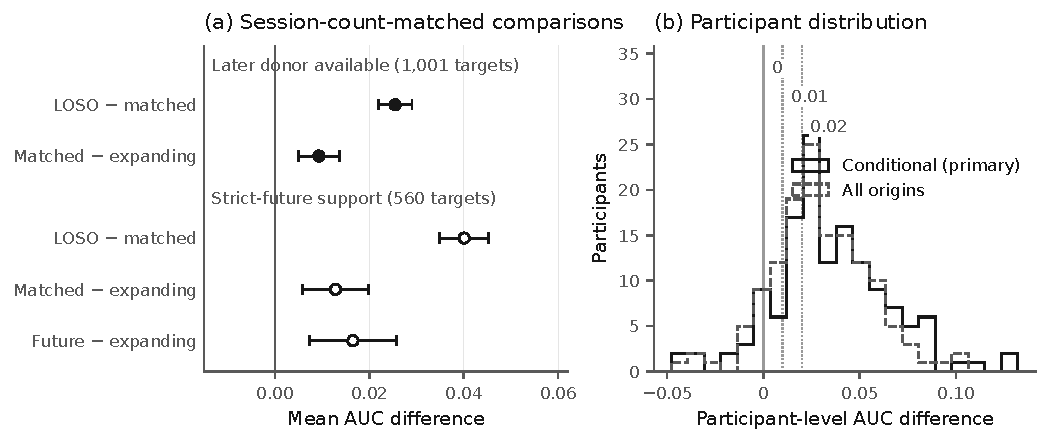
\includegraphics[width=\widefigwidth]{fig2_estimands_distribution.pdf}
\caption{Session-count-matched comparisons and participant distributions.
(a) Session-count-matched comparisons on the conditional support (filled) and
the strict-future support (open); bars are the 95\% confidence intervals of
Table~\ref{tab:common-support}. (b) Participant-level
distributions of the LOSO minus expanding-window difference under the
conditional (primary) and all-origin summaries; the vertical reference lines
mark zero, 0.01, and 0.02 AUC.}
\label{fig:estimands}
\end{figure*}

% Generated by scripts/revision_analysis.py; do not edit.
\begin{table*}[!t]
\centering
\settableformat
\caption{LOSO minus expanding-window AUC under the primary all-origin estimand and the conditional summary. The all-origin estimand includes the final structural zero. Conditional estimates require at least one later session. Target-weighted intervals use a participant-cluster bootstrap.}
\label{tab:estimands}
\begin{tabularx}{0.80\textwidth}{@{}>{\raggedright\arraybackslash}Xrr@{}}
\toprule
Estimand and aggregation & Units & Mean difference [95\% CI] \\
\midrule
All origins, participant-weighted & 138 & +0.030 [+0.025, +0.034] \\
All origins, target-weighted & 138 & +0.030 [+0.026, +0.035] \\
All origins, dataset-weighted & 6 & +0.024 [+0.008, +0.040] \\
All origins, random-effects & 6 & +0.024 [+0.009, +0.039] \\
Conditional, participant-weighted & 138 & +0.035 [+0.030, +0.040] \\
Conditional, target-weighted & 138 & +0.035 [+0.029, +0.040] \\
Conditional, dataset-weighted & 6 & +0.030 [+0.012, +0.047] \\
Conditional, random-effects & 6 & +0.030 [+0.014, +0.046] \\
\bottomrule
\end{tabularx}
\end{table*}


The two decoders agreed on the direction: the conditional difference was
\CSPGapMean{} AUC for CSP+LDA and \TSGapMean{} for TS+LR. LOSO scored higher for
\CondPositive\% of participants, and by more than 0.02 AUC for \CondGtTwo\%
(Table~\ref{tab:practical}).

\subsection{Session-Count-Matched Reference}
\label{sec:partition}
Equation~\eqref{eq:partition} splits the LOSO minus expanding-window difference
into two comparisons, and Table~\ref{tab:common-support} and
Figure~\ref{fig:estimands}(a) report them. Of the \UniformTotalMean{} AUC total on the
1,001 conditional participant--targets, the complete donor set scored
\UniformCountMeanUnsigned{} AUC (95\% CI [\UniformCountLoUnsigned{},
\UniformCountHiUnsigned{}]) above the matched reference, and the matched
reference scored \UniformCompositionMeanUnsigned{} AUC (95\% CI
[\UniformCompositionLoUnsigned{}, \UniformCompositionHiUnsigned{}]) above the
prior-history set. Under this reference,
the two components were about \CondCountShare\% and \CondCompShare\% of the
total.

The 560 early targets with at least $t$ strictly later sessions show the same
pattern on a larger scale. There the total was \StrictTotalMean{} AUC:
\StrictCountMean{} (95\% CI [\StrictCountLo{}, \StrictCountHi{}]) between the
complete donor set and the matched reference, and \StrictCompositionMean{}
(95\% CI [\StrictCompositionLo{}, \StrictCompositionHi{}]) between the matched
reference and the prior-history set. On these targets, an arm trained on $t$ strictly later
sessions scored \StrictFutureMeanUnsigned{} AUC (95\% CI
[\StrictFutureLoUnsigned{}, \StrictFutureHiUnsigned{}]) above the expanding
window. Table~\ref{tab:support} lists
the support of each arm by dataset.

% Generated by scripts/revision_analysis.py; do not edit.
\begin{table*}[!t]
\centering
\settableformat
\caption{Partition of the LOSO minus expanding-window difference under the session-count-matched reference (Equation~\eqref{eq:partition}), on the full conditional support and on the strict-future support required by the future-only arm. The two components sum to the total within each support, up to rounding. All intervals are participant-level $t$ intervals; those involving a sampled arm condition on the five realized donor draws (Appendix~\ref{app:uncertainty}).}
\label{tab:common-support}
\begin{tabularx}{\textwidth}{@{}>{\raggedright\arraybackslash}X S[table-format=3.0] S[table-format=+1.3,retain-explicit-plus=true] r@{}}
\toprule
\textbf{Contrast} & {\textbf{Participants}} & {\textbf{Mean $\boldsymbol{\Delta}$}} & \textbf{95\% CI} \\
\midrule
\multicolumn{4}{@{}l}{\textit{Later donor available: 1,001 participant--targets}} \\
\addlinespace[0.2em]
LOSO $-$ expanding window & 138 & +0.035 & $[+0.030, +0.040]$ \\
LOSO $-$ session-count-matched reference & 138 & +0.025 & $[+0.022, +0.029]$ \\
Session-count-matched reference $-$ expanding window & 138 & +0.009 & $[+0.005, +0.014]$ \\
\addlinespace[0.5em]
\multicolumn{4}{@{}l}{\textit{Strict-future common support: 560 participant--targets}} \\
\addlinespace[0.2em]
LOSO $-$ expanding window & 138 & +0.053 & $[+0.045, +0.061]$ \\
LOSO $-$ session-count-matched reference & 138 & +0.040 & $[+0.035, +0.045]$ \\
Session-count-matched reference $-$ expanding window & 138 & +0.013 & $[+0.006, +0.020]$ \\
Strict future $-$ expanding window & 138 & +0.017 & $[+0.007, +0.026]$ \\
\bottomrule
\end{tabularx}
\end{table*}

% Generated by scripts/revision_analysis.py; do not edit.
\begin{table*}[!t]
\centering
\settableformat
\caption{Observed participant--target support by dataset. The two decoders share these targets. The uniform donor-count-matched reference uses the conditional support; the future-only reference requires strict-future support, $t\leq(T-1)/2$. Mean donor-session count is the target-weighted expanding-window count $t$.}
\label{tab:support}
\begin{tabularx}{0.90\textwidth}{@{}>{\raggedright\arraybackslash}Xrrrr@{}}
\toprule
Dataset & Participants & All origins & Conditional & Strict future \\
\midrule
BNCI2014\_004 & 9 & 36 & 27 & 18 \\
Zhou2016 & 4 & 8 & 4 & 4 \\
Zhou2020 & 20 & 119 & 99 & 59 \\
Kumar2024 & 18 & 90 & 72 & 36 \\
Ma2020 & 25 & 350 & 325 & 175 \\
Stieger2021 & 62 & 536 & 474 & 268 \\
\midrule
Total & 138 & 1139 & 1001 & 560 \\
Mean donor-session count & --- & 5.36 & 4.96 & 2.93 \\
\bottomrule
\end{tabularx}
\end{table*}


\subsection{The Magnitude Varies Across Recording Designs}
The mean difference was positive in all six datasets (Figure~\ref{fig:forest}),
with the widest intervals in the two smallest cohorts, of four and nine
participants.
Weighting the six datasets equally gave a conditional mean of \DatasetMean{}
AUC, and the random-effects estimate was \MetaMean{} (95\% CI [\MetaLo{},
\MetaHi{}]) with $I^2=\MetaI\%$. The prediction interval, [\MetaPredLo{},
\MetaPredHi{}], crosses zero, so a new recording design could show a difference
of either sign even though the average across these designs is positive.
Leaving out one dataset at a time kept the participant-weighted conditional
estimate positive, between \LoDOCondMin{} and \LoDOCondMax{} AUC; without
Stieger2021, the largest cohort, it was \LoDOWithoutStiegerCond{}. Appendix~\ref{app:robust}
breaks the difference down by target position within each dataset.

\begin{figure*}[!t]
\centering
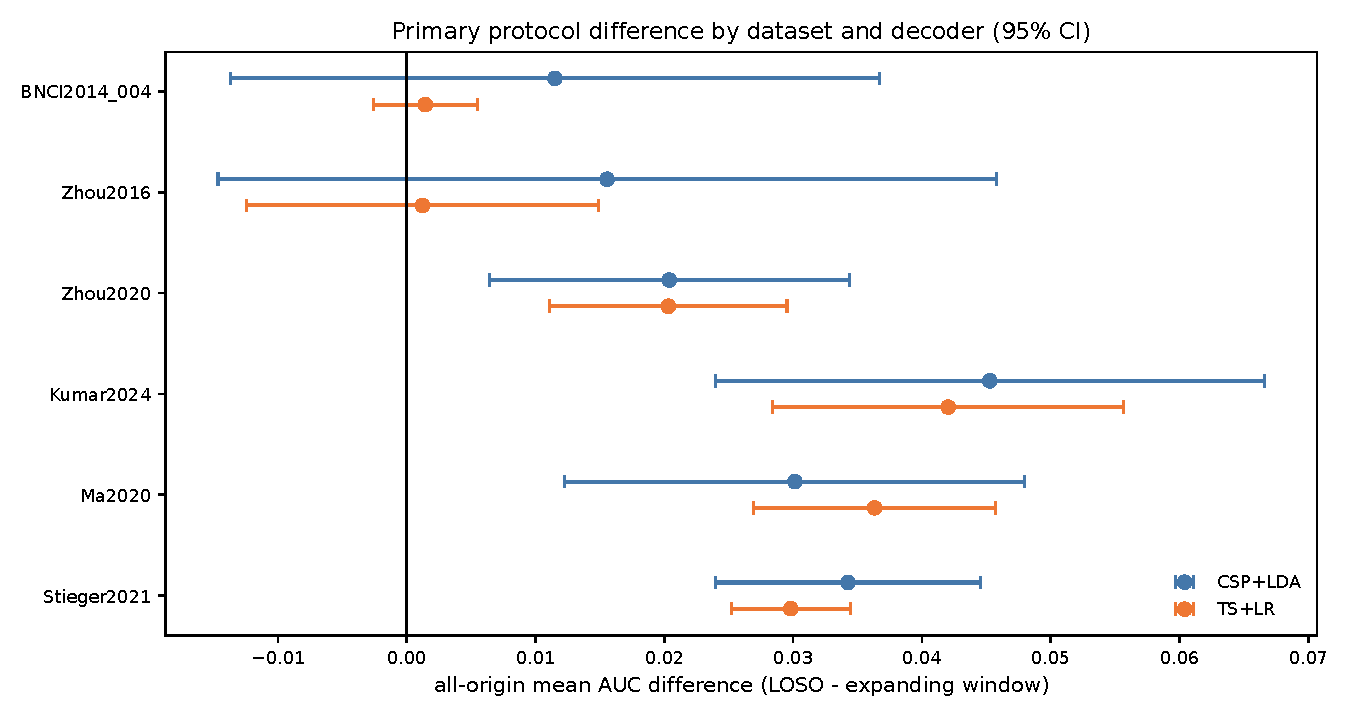
\includegraphics[width=\widefigwidth]{fig1_gap_forest.pdf}
\caption{Conditional LOSO minus expanding-window AUC by dataset and decoder.
Points are dataset means of participant-level contrasts, and bars are 95\%
confidence intervals across participants.}
\label{fig:forest}
\end{figure*}

\subsection{Sensitivity: All-Origin Averaging and Temporal Units}
Including the final targets lowered the pooled estimates as well: under the
all-origin summary, the random-effects estimate was \AllMetaMean{} AUC (95\% CI
[\AllMetaLo{}, \AllMetaHi{}]), and leave-one-dataset-out estimates ranged from
\LoDOAllMin{} to \LoDOAllMax{}. For Ma2020, the conditional difference was \MaBlockCond{} AUC with the released
blocks as units and \MaDayCond{} after the same trials were grouped into three
recording days (Figure~\ref{fig:ma}). The all-origin figures were \MaBlockAll{}
and \MaDayAll{}: Equation~\eqref{eq:zero-scaling} scales the conditional mean by
$13/14$ for blocks but by $1/2$ for days, because the single zero-difference target weighs far more when there are only three units.
Table~\ref{tab:sensitivity} and
Appendix~\ref{app:robust} give the day-level balanced accuracy and the
alternative training policies.

\begin{figure}[t]
\centering
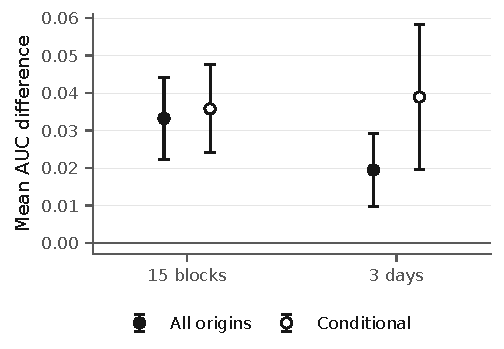
\includegraphics[width=\columnwidth]{fig5_ma_time_unit.pdf}
\caption{Ma2020 sensitivity to the temporal unit. The block analysis uses 15
ordered blocks; the day analysis concatenates five consecutive blocks within each
of three recording days. Bars are 95\% participant-level confidence
intervals.}
\label{fig:ma}
\end{figure}

\subsection{Decoder Rankings and Within-Protocol Margins}
The protocol changed which decoder scored higher for \CondRankChangeN{} of 138
participants (\RankChangePct\%) under the primary estimand. In
\CondFlipCSPtoTSN{} of these, CSP+LDA led under LOSO and TS+LR under the
expanding window; \CondFlipTStoCSPN{} went the other way. Most of these changes
were near ties: only \CondFlipMarginOneN{} of the \CondRankChangeN{} had
decoder differences above 0.01 AUC under both protocols, and under the
all-origin summary the count was \AllFlipMarginOneN{} of \AllRankChangeN{}. TS+LR had the higher mean AUC in all six datasets, under both protocols and both
summaries. Figure~\ref{fig:margins} shows the margins and enlarges the
near-tie region, and Table~\ref{tab:decisions} gives the threshold
sensitivity.

Appendix~\ref{app:eegnet} repeats the ranking comparison for a deep decoder,
using a single-seed EEGNet run on Stieger2021 and a three-seed check on
a fixed 12-participant subset.

\begin{figure*}[!t]
\centering
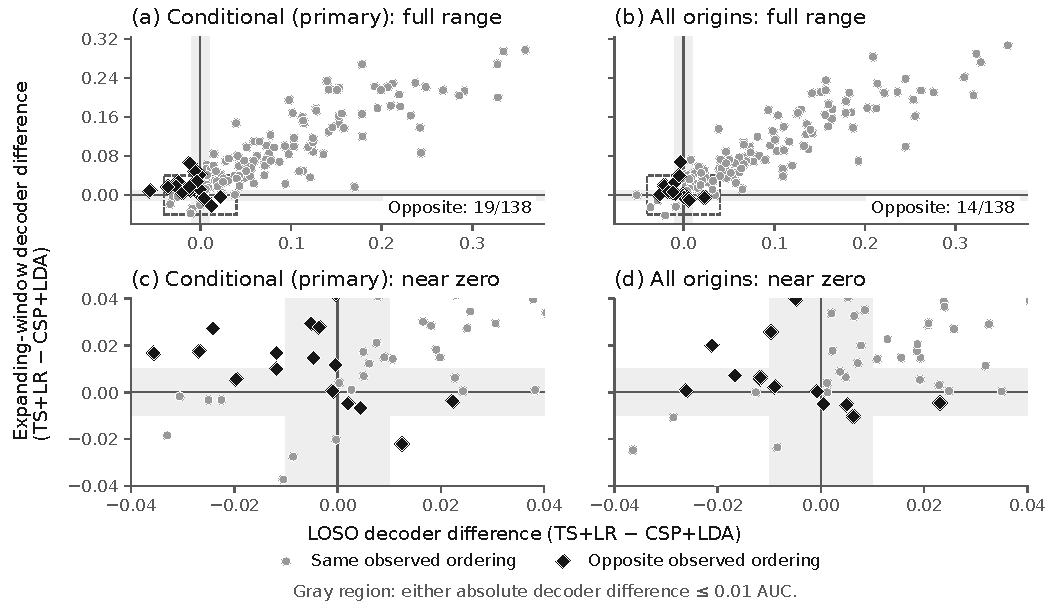
\includegraphics[width=\widefigwidth]{fig6_decoder_margins.pdf}
\caption{Participant-level decoder margins under the two protocols. Each point
is one participant; positive margins favor TS+LR over CSP+LDA. Opposite-sign
quadrants indicate a change in the observed higher-scoring decoder. The upper
panels show the full range; the lower panels enlarge the dashed near-origin
regions using identical limits. Gray circles indicate unchanged ordering and
black diamonds indicate opposite ordering. Shaded bands mark absolute margins at or below 0.01 AUC.}
\label{fig:margins}
\end{figure*}

\section{Discussion}
\label{sec:discussion}
\subsection{Information Sets and the Matched Reference}
With the same test sessions and fixed decoder configurations, LOSO scored
\CondGapMeanUnsigned{} AUC above the expanding window at targets where later sessions
were available. When the LOSO pool was sampled down to the expanding window's
number of sessions, the gap shrank to \UniformCompositionMeanUnsigned{} AUC. Under
this reference, about \CondCountShare\% of the difference lay between the
complete pool and the matched reference, and about \CondCompShare\% between the
matched reference and prior history. The larger share is consistent with the
small-sample behavior of Riemannian classifiers, which degrade when training
trials are few relative to the covariance dimension
\cite{singh2019smallsample}, a condition met at early expanding-window targets
in the high-channel datasets. On early targets with enough future donors, training on
the same number of strictly later sessions also scored higher than training on
prior sessions.

Earlier comparisons stayed within one study or one user
\cite{egger2024chrono,wimpff2025continual,sliwowski2023datasetsize}; here the
comparison covers 138 participants and six recording designs, with an explicit
session-count-matched reference and target-averaging definitions. Because the
size of the difference also varied with the recording design
(Section~\ref{sec:results}-C), a chronological estimate computed for the design
at hand is more informative than a fixed correction applied to LOSO.

\subsection{Consequences for Benchmarking}
MOABB's cross-session evaluation asks how well a decoder performs across the
sessions of one participant \cite{jayaram2018moabb}, and LOSO answers that
question. For a decoder updated from the history available before each session,
expanding-window validation gives the corresponding chronological estimate, and
our paired results show how far apart the two estimates are. A benchmark
addressing both questions can report both; the cross-validator we provide
implements the chronological comparison within MOABB
(Appendix~\ref{app:moabb}).

Target averaging also changes the reported contrast. Including final sessions
lowers the average because it adds structural zeros, and regrouping the Ma2020
blocks into days changes both the update event and the weight of the final
target (Section~\ref{sec:results}-D).

Although the protocols shifted performance levels, the dataset-level order of
CSP+LDA and TS+LR did not change, and participant-level ranking changes occurred
mainly near ties. Comparisons between classical and deep motor-imagery decoders
have been summarized by headline accuracy differences \cite{george2022sota},
which do not show whether the ordering would hold under another protocol. A
benchmark therefore needs separate summaries of how a protocol changes
performance levels and how it changes decoder order. Rankings should come with
their score margins, the participants they cover, and how the training runs
were defined.

\subsection{Reporting Procedure}
A recent review notes that motor-imagery decoding studies often prioritize
accuracy in isolation \cite{raza2025deep}. In BCI Competition IV data,
including the cue-presentation and rest periods in the training data changed
accuracy by more than ten percentage points for some participants, which
complicates comparisons across studies \cite{suemitsu2023visual}. To make such
choices explicit, Table~\ref{tab:reporting} lists five fields that pin down what
a longitudinal estimate represents and fills them in for this analysis. LOSO answers the completed-trajectory question, and the expanding window
answers the chronological one. When both matter, report both, and
name each by what the decoder was allowed to see. In our materials, the result
files identify participant, target, decoder, and protocol, and the support
manifests say which rows and weights enter each estimate.

\begin{table*}[!t]
\centering
\settableformat
\caption{Reporting specification for longitudinal decoding evaluation, with this
analysis as the worked example.}
\label{tab:reporting}
\begin{tabularx}{\textwidth}{@{}>{\raggedright\arraybackslash}p{0.24\textwidth}>{\raggedright\arraybackslash}X@{}}
\toprule
\textbf{Reporting field} & \textbf{Specification in this audit}\\
\midrule
Prediction and update event & A fresh fit before each target session or block;
the Ma2020 day-level analysis fits before each target recording day.\\
\addlinespace[2pt]
Available recordings and labels & Expanding window: all fully labeled prior sessions.
LOSO: all fully labeled sessions other than the target.\\
\addlinespace[2pt]
Target contributions to fitting & No target contributions to learned parameters;
fixed preprocessing followed by scoring on the target trials.\\
\addlinespace[2pt]
Temporal unit and endpoint & Source-defined session or block, through the final
recorded unit; Ma2020 additionally regrouped by recording day.\\
\addlinespace[2pt]
Averaging population & Targets and two decoders averaged within participant, then
participants weighted equally. The primary average uses targets with a later
donor; the all-origin sensitivity summary also includes the final structural
zero. Target-weighted and dataset-weighted summaries are identified separately.\\
\bottomrule
\end{tabularx}
\end{table*}

\section{Conclusion}
Across six motor-imagery datasets and 138 participants, LOSO scored
\CondGapMeanUnsigned{} AUC above expanding-window validation on the same test targets,
where later sessions were available. The difference was positive in every
dataset but varied in size. When the LOSO pool was sampled down to the
expanding window's number of sessions, most of the gap disappeared. The two
decoders kept the same order in every dataset, and participant-level ranking
changes occurred mainly near ties.

A protocol can therefore shift performance levels without changing which
decoder ranks first, so the two need separate summaries. Benchmarks for
decoders retrained before each session should report a chronological estimate
that uses only the history available at each update. They should also state the
update event, temporal unit, and target averaging behind each number, and give
score margins with every ranking.

\section*{Data Availability}
This study is a secondary analysis of the datasets cited in Table~\ref{tab:data}.
Access conditions and raw-data licenses are governed by the original repositories
and dataset publications.

\section*{Code Availability}
The analysis code, manuscript source, and result files will be released at
\url{https://github.com/Yiming-S/loso-vs-prospective-bci}. The materials
include \texttt{Forward\allowbreak Session\allowbreak Splitter}, a
scikit-learn-compatible cross-validator accepting per-trial session labels and
an explicit session order. It implements expanding-window, immediately-previous,
and first-session policies and can be passed to MOABB's
\texttt{Cross\allowbreak Session\allowbreak Evaluation} through the
\texttt{cv\_class} and
\texttt{cv\_kwargs} arguments, so the chronological protocol can be adopted
without modifying the benchmark; Appendix~\ref{app:moabb} reports this check on
BNCI2014\_004. The materials also include version-pinned dependencies, the dataset
registry, inclusion and support manifests, result-level CSV files, seeds,
Stieger reuse provenance, figure sources, and LaTeX source. A result-only
workflow regenerates the classical-decoder analyses and figures without raw
EEG, and an audit checks result coverage, duplicate keys, score ranges, and
final-origin structural zeros. Raw-cache checks, including epoch length and
retained channels, require the original recordings or local caches.

\section*{Ethics Statement}
The analysis uses previously released, de-identified datasets and collects no new
human-participant data. Ethical approvals and consent procedures are reported in the
original dataset publications.

\section*{Author Contributions}
Yiming Shen: conceptualization, methodology, software, validation, formal analysis,
data curation, visualization, writing---original draft, and writing---review and
editing.

\section*{Funding and Acknowledgment}
This research received no external funding. OpenAI Codex assisted with structural
and language editing throughout the manuscript,
analysis-code revision for Sections IV--V and the appendices, figure generation,
and LaTeX formatting. The author is responsible for the scientific content,
numerical results, citations, and final manuscript.

\appendices
\section{Robustness and Interpretation Checks}
\label{app:robust}

\subsection{Participant-Level Ranking and Threshold Sensitivity}
The primary participant-level median was \CondMedian{} AUC (IQR
[\CondIQRLo{}, \CondIQRHi{}]). Table~\ref{tab:practical} reports how many participants had a positive
difference and how many exceeded each threshold.
Table~\ref{tab:decisions} reports observed ranking changes, margin sensitivity,
and threshold crossings in both directions.

% Generated by scripts/revision_analysis.py; do not edit.
\begin{table}[!t]
\centering
\settableformat
\caption{Observed participant-level magnitude and counts, $n$ (\%), of the protocol difference.}
\label{tab:practical}
\begin{tabularx}{\columnwidth}{@{}>{\raggedright\arraybackslash}Xrr@{}}
\toprule
Metric & All origins & Conditional \\
\midrule
Median [IQR] & +0.026 [+0.014, +0.046] & +0.031 [+0.017, +0.053] \\ 
Participants with $\Delta>0$ & 124 (89.9\%) & 124 (89.9\%) \\
Participants with $\Delta>0.01$ & 113 (81.9\%) & 115 (83.3\%) \\
Participants with $\Delta>0.02$ & 92 (66.7\%) & 98 (71.0\%) \\
\bottomrule
\end{tabularx}
\end{table}

% Generated by scripts/revision_analysis.py; do not edit.
\begin{table}[!t]
\centering
\settableformat
\caption{Observed participant-specific decoder ordering and illustrative threshold crossings ($n=138$). Arrows go from LOSO to expanding-window ordering. Bilateral margins require both absolute TS+LR-minus-CSP+LDA mean AUC differences to exceed the threshold. Threshold crossings average both decoders and targets within participant. These are descriptive point-estimate comparisons.}
\label{tab:decisions}
\begin{tabularx}{\columnwidth}{@{}>{\raggedright\arraybackslash}Xrr@{}}
\toprule
Outcome & All origins & Conditional \\
\midrule
Opposite decoder ordering & 14 (10.1\%) & 19 (13.8\%) \\ 
CSP+LDA $\to$ TS+LR & 10 & 15 \\ 
TS+LR $\to$ CSP+LDA & 4 & 4 \\ 
Flip, both margins $>0.005$ & 7 & 11 \\
Flip, both margins $>0.01$ & 1 & 6 \\
Flip, both margins $>0.02$ & 1 & 1 \\
LOSO-only AUC $\geq0.70$ & 13 & 16 \\ 
Expanding-only AUC $\geq0.70$ & 1 & 1 \\ 
LOSO-only AUC $\geq0.75$ & 22 & 31 \\ 
Expanding-only AUC $\geq0.75$ & 0 & 0 \\ 
\bottomrule
\end{tabularx}
\end{table}


\subsection{Target Position and Later-Session Availability}
Figure~\ref{fig:history} plots the conditional difference against the number of
later sessions that only LOSO could use. This count equals $T_i-1-t$, so each
curve mixes target position, accumulated history, and trajectory length. The
curves differ by dataset; in several of the longer trajectories the early
targets show the larger differences.

\begin{figure*}[!t]
\centering
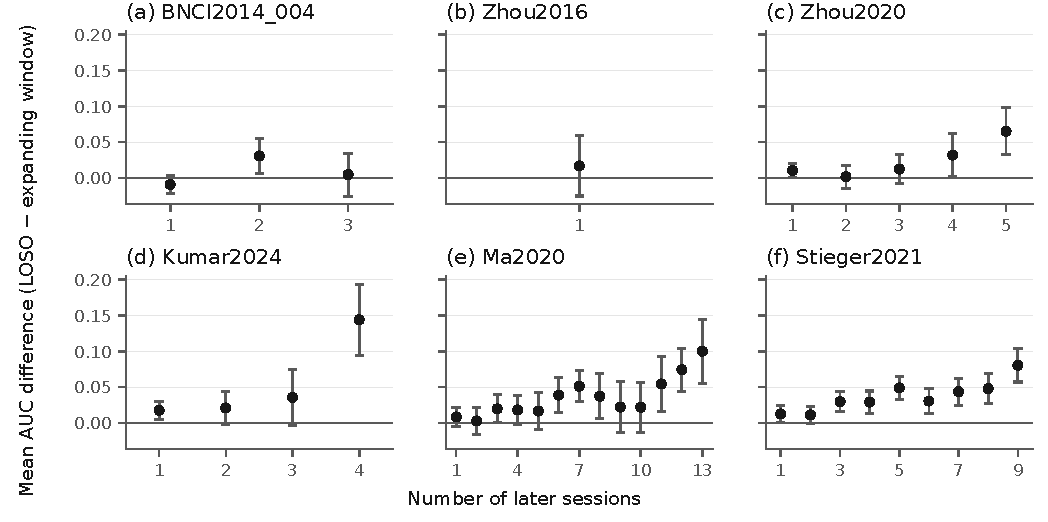
\includegraphics[width=\widefigwidth]{fig3_history_by_dataset.pdf}
\caption{Dataset-specific association between the protocol difference and the
number of later sessions available to LOSO. Each point averages participants and
both decoders at a common within-dataset index; bars are 95\% participant-level
confidence intervals.}
\label{fig:history}
\end{figure*}

\subsection{Ma2020 Temporal Unit}
Table~\ref{tab:sensitivity} gives the Ma2020 block- and day-level estimates
alongside two alternative training policies. On the day-level conditional support,
the balanced-accuracy
difference was \MaDayBA{} (95\% CI [\MaDayBALo{}, \MaDayBAHi{}]).

% Generated by scripts/revision_analysis.py; do not edit.
\begin{table}[!t]
\centering
\settableformat
\caption{Alternative training policies and Ma2020 time-unit sensitivity.}
\label{tab:sensitivity}
\par\smallskip
\begin{tabularx}{\columnwidth}{@{}>{\raggedright\arraybackslash}X S[table-format=3.0] r@{}}
\toprule
\textbf{Analysis} & {$\boldsymbol{n}$} & \shortstack[r]{\textbf{Mean $\boldsymbol{\Delta}$}\\\textbf{95\% CI}} \\
\midrule
\multicolumn{3}{@{}l}{\textit{Alternative policies (conditional targets): LOSO minus}} \\
Immediately previous session & 138 & $+0.066\;[+0.058, +0.074]$ \\
First session & 138 & $+0.103\;[+0.091, +0.116]$ \\
\addlinespace[0.4em]
\multicolumn{3}{@{}l}{\textit{Ma2020: blocks}} \\
All origins & 25 & $+0.033\;[+0.022, +0.044]$ \\
Conditional & 25 & $+0.036\;[+0.024, +0.048]$ \\
\addlinespace[0.4em]
\multicolumn{3}{@{}l}{\textit{Ma2020: days}} \\
All origins & 25 & $+0.019\;[+0.010, +0.029]$ \\
Conditional & 25 & $+0.039\;[+0.020, +0.058]$ \\
\bottomrule
\end{tabularx}
\end{table}


\subsection{Adjacent Covariance-Distance Proxy}
Regressing the target-level contrast on the standardized distance between the
unconditional mean covariances of adjacent sessions gave a participant-clustered
coefficient of \DriftRobustBeta{} AUC (95\% CI [\DriftRobustLo{},
\DriftRobustHi{}], $p \DriftRobustP$). Ninety-one of 2,002 target--decoder
observations exceeded the Cook's-distance threshold; removing them produced a
similarly near-zero association.

\subsection{EEGNet Case Study and Seed Sensitivity on Stieger2021}
\label{app:eegnet}
We also analyzed an existing EEGNet run on Stieger2021 ($n=62$, seed 20260716)
that used the same filtering, resampling, epoching, and target definitions, with
a seeded NumPy \texttt{RandomState} and PyTorch seed set before each fit.
EEGNet \cite{lawhern2018eegnet} used the standard compact configuration
($F_1=8$, $D=2$, $F_2=16$, temporal kernel 64, dropout 0.25), trained with Adam
(learning rate $10^{-3}$, weight decay $10^{-4}$, batch size 32) for at most 250
epochs with early stopping (patience 40). Per-channel means and standard
deviations were fitted on all donor trials. The donor trials were then randomly
permuted, and $\max(2,\operatorname{round}(0.15n_{\mathrm{donor}}))$ of them
were held out for validation with the rest used for optimization; if either
subset had fewer than two classes, the complete donor pool served both. Early stopping monitored validation cross-entropy (minimum
improvement $10^{-4}$) and retained the best weights. No target trials
contributed to standardization, fitting, or model selection.

\begin{table}[!t]
\centering
\settableformat
\caption{Illustrative Stieger2021 analysis ($n=62$, seed 20260716):
participant-weighted mean AUC over common targets and the all-origin protocol
difference. Bold entries identify the higher-scoring decoder.}
\label{tab:eegnet}
\begin{tabularx}{\columnwidth}{@{}>{\raggedright\arraybackslash}X *{3}{S[table-format=+1.3]}@{}}
\toprule
\textbf{Protocol} & {\textbf{CSP+LDA}} & {\textbf{TS+LR}} & {\textbf{EEGNet}} \\
\midrule
LOSO & 0.730 & 0.861 & \bfseries 0.882 \\
Expanding window & 0.696 & \bfseries 0.831 & 0.801 \\
\addlinespace[2pt]
LOSO $-$ expanding window & +0.034 & +0.030 & +0.081 \\
\bottomrule
\end{tabularx}
\end{table}

Table~\ref{tab:eegnet} reports the result; paired comparisons use participant
mean differences over common targets with two-sided $t$ intervals and tests.
Under LOSO, EEGNet scored 0.021 AUC above TS+LR (95\% CI [0.006, 0.036], paired
$p=0.007$). Under the expanding window the order flipped: TS+LR scored 0.031 AUC
above EEGNet (95\% CI [0.014, 0.047], $p<0.001$). The protocol difference was
largest for EEGNet, +0.081 AUC, roughly 2.5 times that of either classical
decoder (+0.034 and +0.030). At the participant level the EEGNet-versus-TS+LR
winner changed for 25 of 62 participants, and for 16 of them both
within-protocol margins exceeded 0.01 AUC.

For the seed check we took a fixed random subset of 12 participants (seed
20260716), six with seven sessions and six with eleven, and retrained EEGNet
with seeds 20260716, 20260717, and 20260718 on the same device and
configuration. Each run was compared with TS+LR on the same participants and
common targets ($t\geq1$), averaging targets within participant and then
weighting participants equally (Table~\ref{tab:eegnet-seeds}). TS+LR scored
higher under the expanding window at all three seeds, while the LOSO
differences ranged from $-0.0055$ to $+0.0005$ AUC, inside the 0.01 near-tie
band. At seed 20260716 the subset's scores match the full-cohort records.

\begin{table}[!t]
\centering
\settableformat
\caption{EEGNet-minus-TS+LR mean AUC on the same fixed Stieger2021 subset
($n=12$), with participants weighted equally over common targets. Positive
values favor EEGNet.}
\label{tab:eegnet-seeds}
\begin{tabularx}{\columnwidth}{@{}X *{2}{S[table-format=-1.4]}@{}}
\toprule
\textbf{Training seed} & {\textbf{LOSO}} & {\shortstack{\textbf{Expanding}\\\textbf{window}}} \\
\midrule
20260716 & -0.0055 & -0.0635 \\
20260717 & -0.0030 & -0.0534 \\
20260718 & +0.0005 & -0.0505 \\
\bottomrule
\end{tabularx}
\end{table}

\subsection{MOABB Integration Check}
\label{app:moabb}
To check that the chronological protocol runs inside the unmodified benchmark,
we handed the cross-validator to MOABB 1.5.0 by setting
\texttt{cv\_class} to \texttt{Forward\allowbreak Session\allowbreak Splitter}
and \texttt{cv\_kwargs} to \texttt{\{'mode': 'expanding'\}} in
\texttt{Cross\allowbreak Session\allowbreak Evaluation}, and ran BNCI2014\_004
with the same paradigm settings (8--35 Hz, $[0,3)$ s, 128 Hz) and the two fixed
decoders. The benchmark, with no change to its evaluation code, produced one
score per target session $t\geq1$: four expanding-window splits per
participant, 36 scores per decoder, 72 in total. These agreed with the
manuscript's expanding-window AUCs for the same participant, target, and decoder
to within 0.004 AUC (mean absolute difference below 0.001), and the benchmark's
default LOSO run agreed with the manuscript's LOSO AUCs to the same degree. The
small residual comes from epoch length: the benchmark keeps the sample at
exactly 3 s (385 samples), whereas the audited loader crops to 384. Mean AUC
over the 36 participant--targets was 0.784 for CSP+LDA and 0.808 for TS+LR in
both implementations. The script and its per-session comparison table are part
of the analysis materials.

\section{Interval Definitions and Donor-Sampling Uncertainty}
\label{app:uncertainty}
\subsection{Dataset-Level Synthesis}
Let $y_d$ and $v_d$ be the participant mean and its estimated sampling variance
for dataset $d$, and let $k=6$. With restricted-maximum-likelihood estimate
$\widehat\tau^2$, the weights and pooled mean are
\begin{equation}
w_d=(v_d+\widehat\tau^2)^{-1},\qquad
\widehat\mu=\frac{\sum_d w_d y_d}{\sum_d w_d}.
\end{equation}
The reported mean interval uses the unscaled standard error and is
$\widehat\mu\pm t_{k-1,0.975}(\sum_d w_d)^{-1/2}$. The approximate prediction
interval \cite{higgins2009reevaluation} is
$\widehat\mu\pm t_{k-2,0.975}
\sqrt{\widehat\tau^2+(\sum_d w_d)^{-1}}$.
For the Hartung--Knapp--Sidik--Jonkman sensitivity analysis
\cite{rover2015hartung}, define
$q=\sum_d w_d(y_d-\widehat\mu)^2/(k-1)$ and replace the mean standard error
by $\sqrt{q/\sum_d w_d}$. This gives intervals of
[\AllMetaHKLo{}, \AllMetaHKHi{}] for all origins and
[\CondMetaHKLo{}, \CondMetaHKHi{}] for conditional targets.

\subsection{Donor-Sampling Uncertainty of the Matched Reference}
The matched reference averages each row's AUC over $B=5$ random donor draws, so
the participant scatter behind the matched-reference intervals contains draw
noise as well as participant variation; the unsampled LOSO--expanding contrast
is untouched by the draws. Here we bound the draw part. The cached
standard deviation $s_{r,0}$ of each row's AUC across the draws uses divisor
$B$, so the standard error of the row's draw mean is $e_r=s_{r,0}/\sqrt{B-1}$. The participant-weighted contrast is $\sum_r a_r
\bar x_r$ with nonnegative weights $a_r$ summing to one (equal participants,
then equal targets and decoders within participant). Each participant draws
from its own seed, so draw errors are independent across participants; only
\SharedSeedPairs{} of \SubjectTPairs{} participant--length pairs share a draw
pattern across datasets. The intervals of Table~\ref{tab:common-support} are
computed from that scatter and are not adjusted for a shared draw component. Per-draw AUCs were
not stored, so the covariance of draw errors across rows is not identifiable
from the cached summaries. Under
independent draws across targets, with the two decoder rows of one target
treated as perfectly correlated, the donor-sampling component of the aggregate
standard error is \CondCompDrawSE{} AUC on the conditional support and
\StrictCompDrawSE{} on the strict-future support, against a participant-level
standard error of \CondCompParticipantSE{} for the matched-minus-expanding
contrast. The covariance-agnostic bound $\sum_r a_r e_r$ equals
\CondMatchedTriangleSE{} and \StrictMatchedTriangleSE{} AUC on the two
supports.

% Balance the references and biography on the final two-column page.
\balance
\bibliographystyle{IEEEtran}
\bibliography{references}

% Keep the biography intact when the final columns are balanced.
\noindent\begin{minipage}{\columnwidth}
\begin{IEEEbiography}[{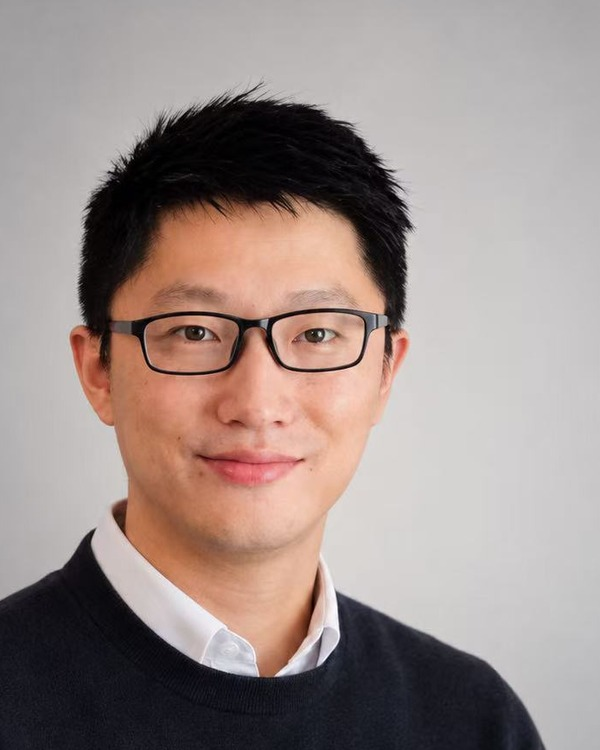
\includegraphics[width=1in,height=1.25in,clip,keepaspectratio]{yiming_shen.jpg}}]{Yiming Shen}
received the Ph.D. degree in computational sciences from the University of
Massachusetts Boston, Boston, MA, USA, in 2026.

Dr. Shen has prior industry experience managing sensor time-series data and
develops open-source Python and R tools for cross-session EEG transfer
experiments, benchmark inspection, distribution-shift diagnostics, and
covariance-based feature extraction. Dr. Shen's research interests include
electroencephalography-based brain--computer interfaces, the evaluation of EEG
decoding systems, transfer across recording sessions and participants,
accuracy--cost trade-offs in decoder selection, and reproducible statistical
learning.\EOD
\end{IEEEbiography}
\end{minipage}
\end{document}
